\chapter{Kode Analisis Benchmark Write}
\label{appendix:write-benchmark-code}

Lampiran ini menunjukkan kode yang digunakan untuk melakukan visualisasi dari hasil \textit{benchmark} pada skenario \textit{write} dengan \textit{payload} besar dan \textit{bandwidth} internet menengah. Kode ini bertujuan untuk memperlihatkan proses yang dilakukan untuk menghasilkan grafik dan diagram dalam analisis. Analisis dilakukan dengan menggunakan kakas Jupyter Notebook dan bahasa pemrograman Python, dengan pustaka seperti NumPy, Pandas, Matplotlib, dan Seaborn.

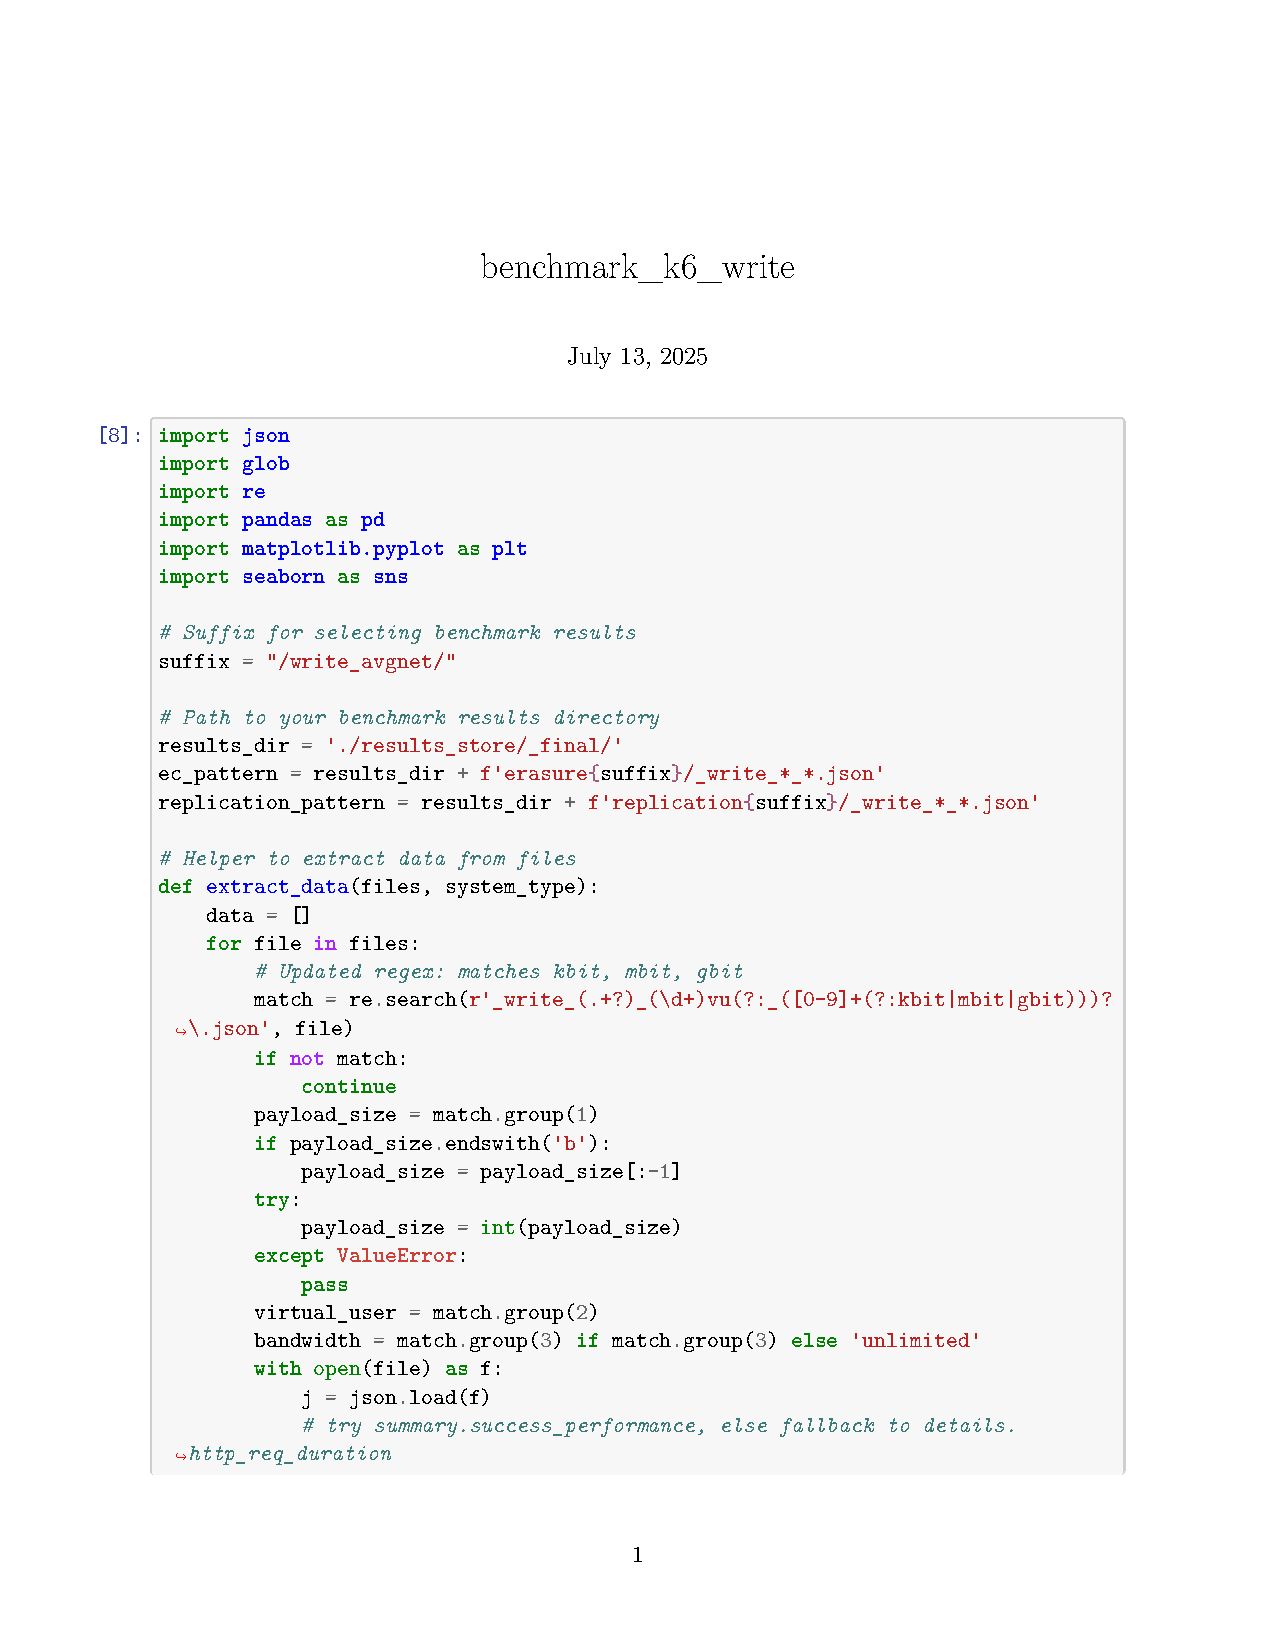
\includepdf[pages=-]{resources/appendix/benchmark_k6_write.pdf}